\section{Front-End Implementation}
Il FrontEnd fornisce delle schermate finalizzate alla fruizione dei quiz, altre finalizzate alla gestione degli utenti ed infine due schermate ausiliarie: una che fornisce informazioni sugli alfabeti e una che mostra l’attuale classifica in base ai punteggi accumulati dagli utenti.


\begin{figure}[!h]
\centering
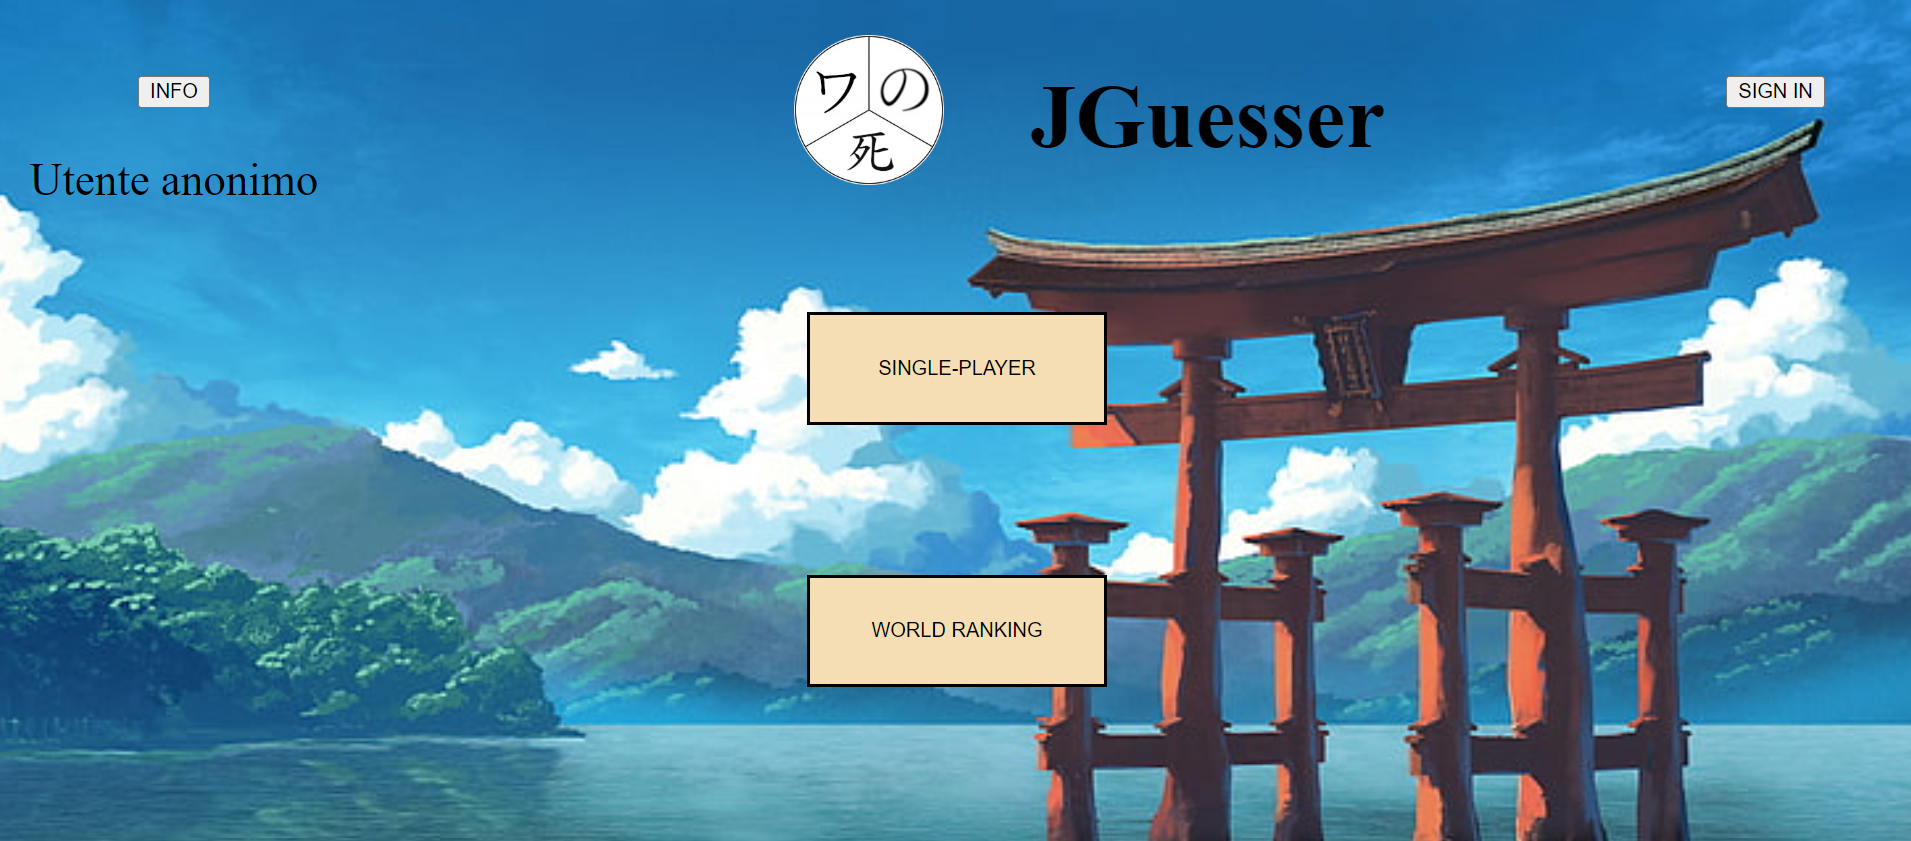
\includegraphics[scale=0.40]{images/homeUnlogged.png}
\caption{Schermata home per utenti non loggati}
\label{fig:user_flow_guest}
\end{figure}
\noindent


\begin{figure}[!h]
\centering
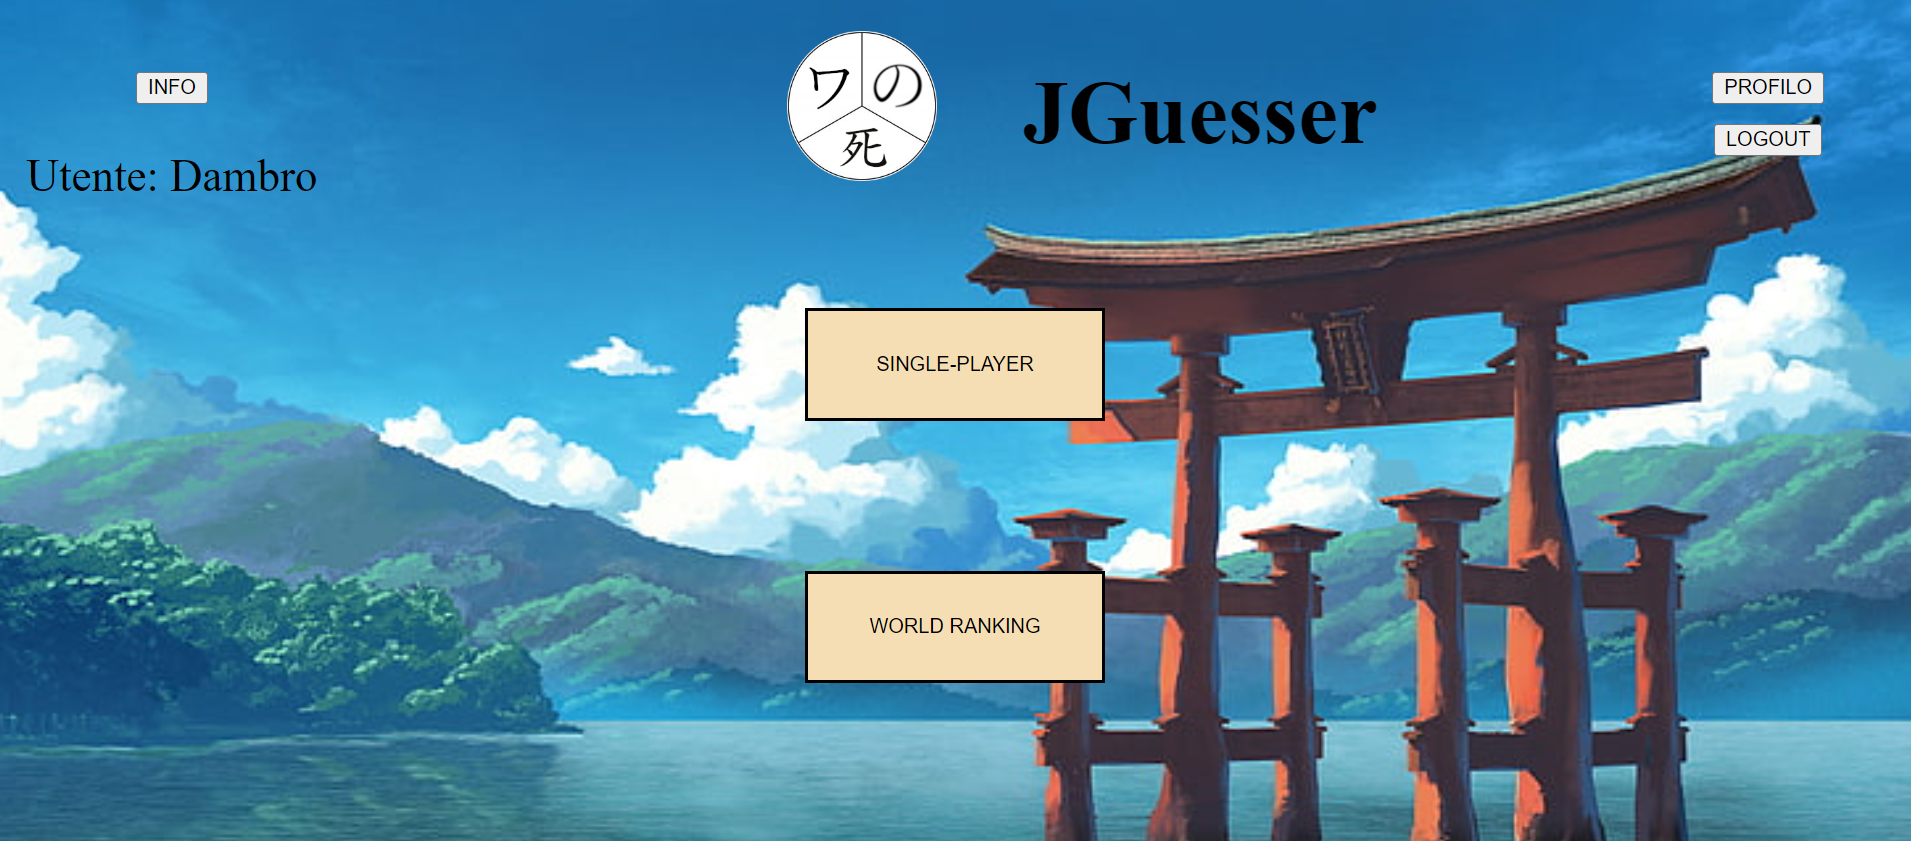
\includegraphics[scale=0.40]{images/homeLogged.png}
\caption{Schermata home per utenti loggati}
\label{fig:user_flow_guest}
\end{figure}
\noindent

\begin{figure}[!h]
\centering
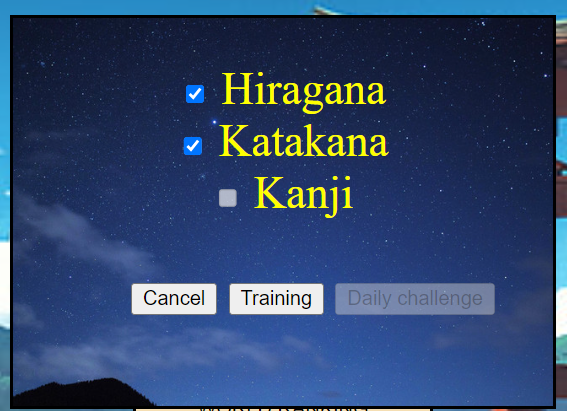
\includegraphics[scale=0.80]{images/sceltaAlfabetoUnlogged.png}
\caption{Scelta modalità di gioco per utenti non loggati}
\label{fig:user_flow_guest}
\end{figure}
\noindent

\begin{figure}[!h]
\centering
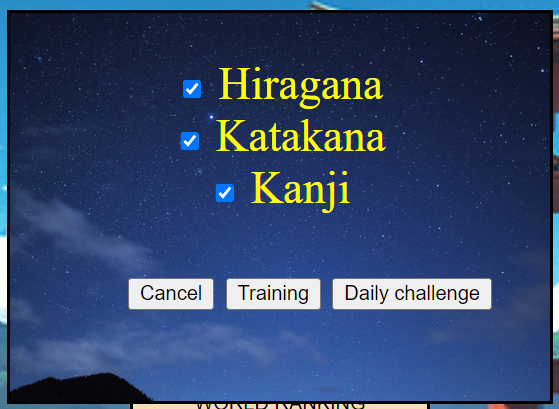
\includegraphics[scale=0.80]{images/sceltaAlfabetoLogged.png}
\caption{Scelta modalità per utenti loggati}
\label{fig:user_flow_guest}
\end{figure}
\noindent


All’interno della home page è possibile trovare le seguenti opzioni:
\begin{itemize}
    \item Pulsante “INFO”: da tale pulsante sarà possibile accedere ad una schermata mostrante informazioni riguardanti gli alfabeti presenti all’interno dell’applicazione. Al di sotto sarà riportato il nome dell'utente (nel caso di utente loggato) oppure "Utente anonimo"
    \item Pulsante “SINGLE-PLAYER”: attraverso tale pulsante si aprirà una finestra di dialogo (figura 29 o figura 30) che permetterà all’utente di scegliere tra 2 (utente non loggato) o 3 (utente loggato) alfabeti. L’utente non loggato avrà inoltre a disposizione soltanto la modalità di “Training”, mentre l’utente loggato avrà a disposizione la “Daily challenge”, da eseguire massimo una volta al giorno.
    Il pulsante “Cancel” chiuderà la finestra di dialogo, mostrando nuovamente la schermata home.
    \item Pulsante “WORLD RANKING”: cliccando su questo pulsante sarà possibile visualizzare la classifica degli utenti (figura 31).
    \item A seconda del fatto che l’utente sia loggato o meno, in alto a destra della schermata home compariranno pulsanti differenti:
    \begin{itemize}
        \item SIGN IN: l’utente non loggato verrà reindirizzato alla schermata di login (figura 33)
        \item PROFILO: l’utente loggato potrà visualizzare dati e statistiche personali (figura 36), permettendo inoltre la modifica di email e password
        \item LOGOUT: l’utente loggato verrà reindirizzato alla schermata home (figura 27) e le sue credenziali verranno dimenticate
    \end{itemize}
\end{itemize}


\begin{figure}[!h]
\centering
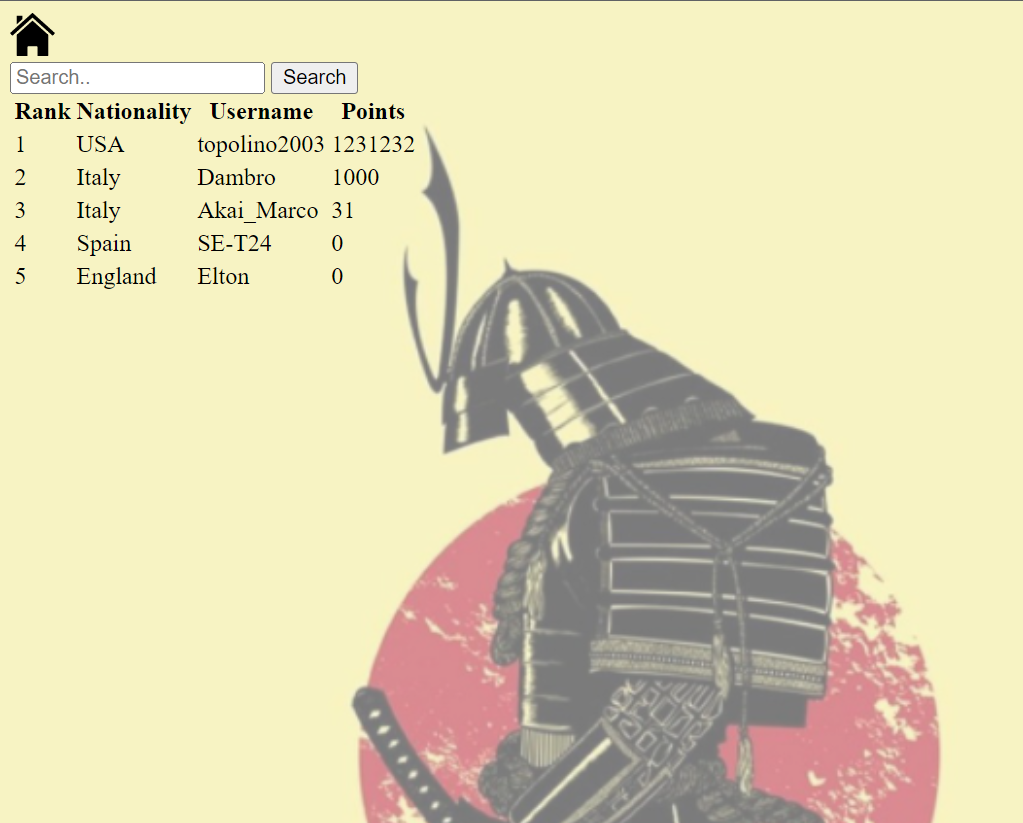
\includegraphics[scale=0.70]{images/classifica.png}
\caption{Classifica}
\label{fig:user_flow_guest}
\end{figure}
\noindent


\begin{figure}[!h]
\centering

\includegraphics[scale=0.70]{images/classificaFiltrata.png}
\caption{Classifica}
\label{fig:user_flow_guest}
\end{figure}
\noindent


\begin{figure}[!h]
\centering
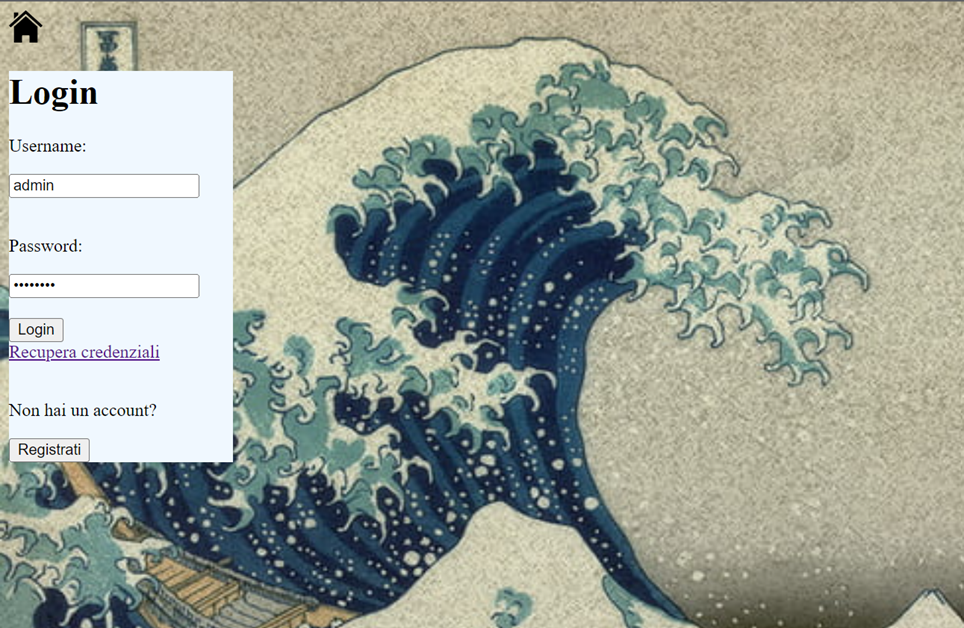
\includegraphics[scale=0.70]{images/login.png}
\caption{Schermata di login}
\label{fig:user_flow_guest}
\end{figure}
\noindent


\begin{figure}[!h]
\centering

\includegraphics[scale=0.70]{images/recuperaCredenziali.png}
\caption{Recupero credenziali}
\label{fig:user_flow_guest}
\end{figure}
\noindent


\begin{figure}[!h]
\centering
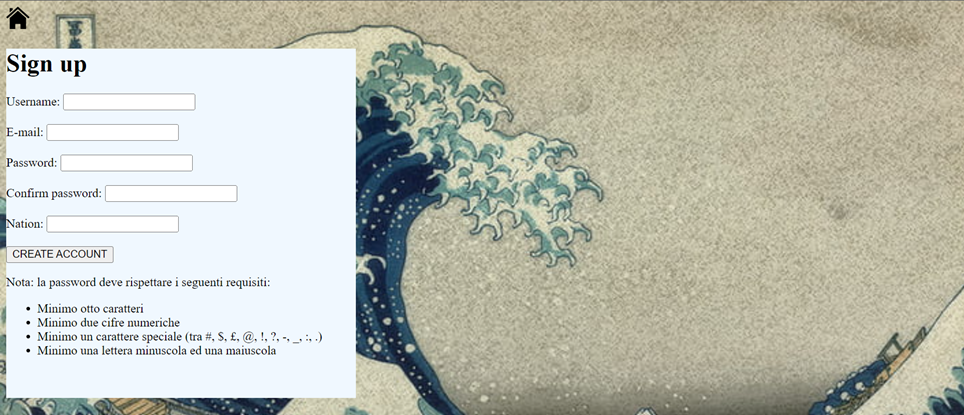
\includegraphics[scale=0.70]{images/signUp.png}
\caption{Schermata di registrazione}
\label{fig:user_flow_guest}
\end{figure}
\noindent
\newpage
Dalla schermata di login sarà possibile, dopo aver inserito le proprie credenziali e cliccato sul pulsante “LOGIN”, visualizzare la schermata home da utente loggato (figura 28).
Nel caso non si ricordino le credenziali, sarà possibile, inserendo l’email associata all’account, ottenere via mail le proprie credenziali (figura 34).
Dalla schermata di login sarà inoltre possibile registrarsi, cliccando sull’apposito pulsante “Registrati” e compilando i relativi campi (figura 35)

\begin{figure}[!h]
\centering
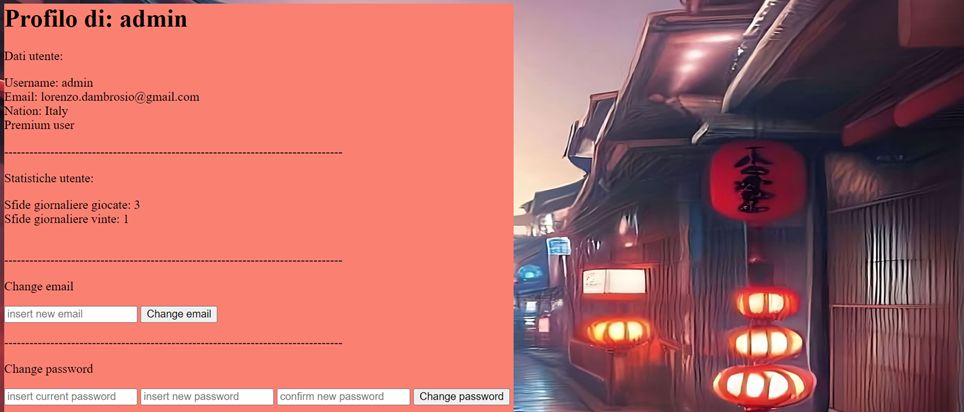
\includegraphics[scale=0.70]{images/profilo.png}
\caption{Schermata profilo utente}
\label{fig:user_flow_guest}
\end{figure}
\noindent

Una volta giunto alla schermata relativa al proprio profilo, l’utente potrà visualizzare i propri dati personali e le proprie statistiche, inoltre, compilando i relativi form, potrà modificare la propria email o la propria password.


\begin{figure}[!h]
\centering

\includegraphics[scale=0.70]{images/quiz1.png}
\label{fig:user_flow_guest}
\end{figure}
\noindent


\begin{figure}[!h]
\centering
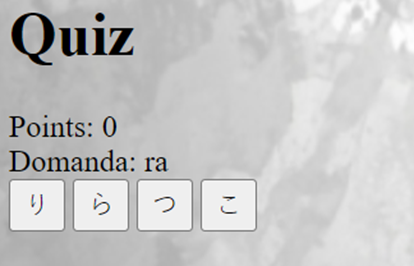
\includegraphics[scale=0.70]{images/quiz2.png}
\caption{Schermata di quiz}
\label{fig:user_flow_guest}
\end{figure}
\noindent


\begin{figure}[!h]
\centering
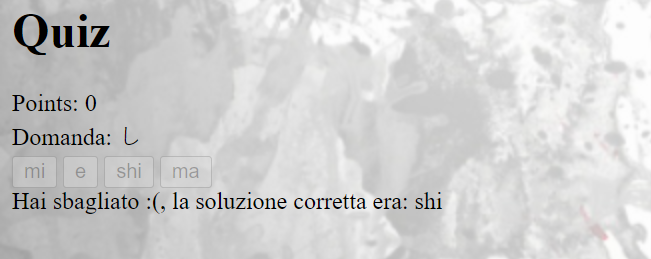
\includegraphics[scale=0.70]{images/quizErrato.png}
\caption{Schermata di quiz, risposta errata}
\label{fig:user_flow_guest}
\end{figure}
\noindent


\begin{figure}[!h]
\centering

\includegraphics[scale=0.70]{images/quizCorretto.png}
\caption{Schermata di quiz, risposta esatta}
\label{fig:user_flow_guest}
\end{figure}
\noindent


\begin{figure}[!h]
\centering
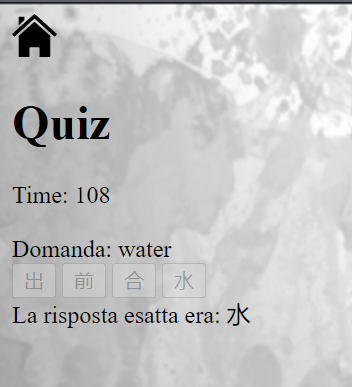
\includegraphics[scale=0.70]{images/dailyChallengeCorretta.png}
\caption{Schermata quiz, daily challenge}
\label{fig:user_flow_guest}
\end{figure}
\noindent


\begin{figure}[!h]
\centering
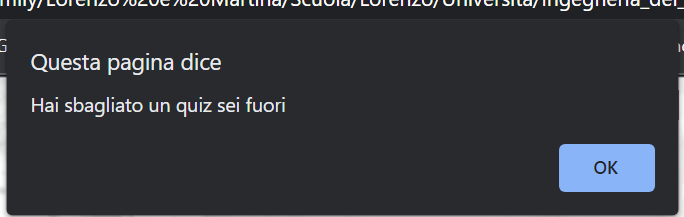
\includegraphics[scale=0.70]{images/dailyChallengeErrore.png}
\caption{Schermata quiz, errore daily challenge}
\label{fig:user_flow_guest}
\end{figure}
\noindent


Selezionando una delle due modalità di gioco (figura 29/30) l’utente visualizzerà una schermata contenente un quiz generato casualmente (in caso di training) o relativo al quiz prescelto per la sfida giornaliera (in caso di daily challenge).
Una volta visualizzata la schermata, l’utente dovrà selezionare (o digitare, a seconda della tipologia di quiz) la risposta che ritiene corretta (eventualmente premendo INVIA RISPOSTA).
A questo punto il sistema comunicherà all’utente se la risposta selezionata è errata (figura 38) o corretta (figura 39), in quest’ultimo caso il punteggio andrà ad incrementarsi. La schermata rimarrà invariata per 3 secondi, per poi lasciar spazio al quiz successivo.
Per terminare la partita, all’utente basterà premere il pulsante home presente in alto a sinistra (figura 37) per essere reindirizzato alla schermata di home (figura 27/28). Il sistema provvederà ad aggiornare il punteggio ottenuto nel training o nella sfida giornaliera, segnando quest’ultima come completata. Sarà possibile effettuare una nuova partita nella modalità “daily challenge” a partire dalla mezzanotte dello stesso giorno.
Nel caso della sfida giornaliera, quest’ultima terminerà al compimento di essa, o in seguito ad un certo quantitativo di errori (in base alla tipologia di sfida prestabilita), il tutto segnalato all’utente (figura 41)
